\section{Resultados}


\subsection{Resultados por módulo}


\subsection{Temperatura}
El circuito final de esta consigna del laboratorio se puede ver en la imagen correspondiente. 

\paragraph{Envío de datos por USART}

En la Figura \ref{fig:Tem_USART} se puede observar la forma en la que se enviaban los datos por puerto serial entre el \texttt{ATmega328P} y el código de Python. 

\begin{figure}[H]
    \centering
    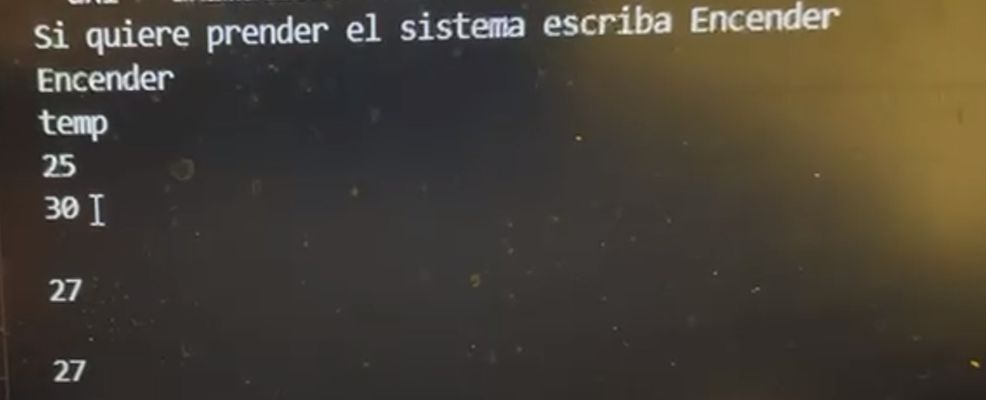
\includegraphics[width=0.35\textwidth]{anexos/2 Temperatura/USART Temperatura.png}
    \caption{Comunicación de datos vía USART entre el microcontrolador y Python.}
    \label{fig:Tem_USART}
\end{figure}

\paragraph{Gráfica en tiempo real}

El resultado de la gráfica en tiempo real se muestra en la Figura \ref{fig:Grafica1}. En ella se observa cómo el eje X representa la evolución temporal de la ejecución (hora de registro en tiempo real), mientras que en el eje Y se visualizan los valores de temperatura obtenidos cada segundo.  
Además, se incluye una línea de referencia que indica la temperatura media esperada.

\begin{figure}[H]
    \centering
    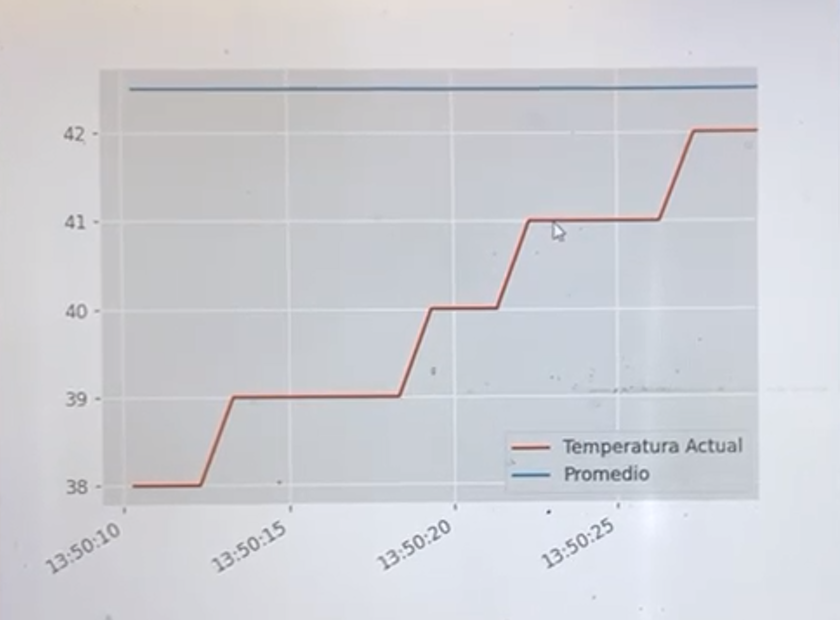
\includegraphics[width=0.35\textwidth]{anexos/2 Temperatura/Grafica tiempo real.png}
    \caption{Gráfica de temperatura en tiempo real.}
    \label{fig:Grafica1}
\end{figure}

\paragraph{Simulación}

Véase la Figura  para una representación del montaje de la simulación, la cual fue realizada en el entorno \textbf{Proteus}. En dicha figura se puede observar la disposición de los componentes utilizados y las conexiones correspondientes al sistema de control térmico.

\paragraph{Gráfica de la simulación}

El resultado de la gráfica correspondiente a la simulación se muestra en la Figura .  
De manera análoga a la gráfica en tiempo real, se presentan en una misma figura tanto la temperatura de referencia como la temperatura medida en cada instante de tiempo.  
La diferencia principal radica en que en esta gráfica se visualiza la **línea temporal completa** de toda la simulación.
